\documentclass[12pt]{article}
\usepackage[utf8]{inputenc}

\RequirePackage{fix-cm}         % para setear tamaños de subindices
\DeclareMathSizes{12}{12}{7}{4}


\pretolerance=5000
\tolerance=9000
\emergencystretch=8pt

\usepackage{lipsum}             % lorem ipsum

\usepackage{blindtext}          % para usar en lugar de lorem ipsum

% cursivas
% \usepackage{fontspec}
% \setmainfont{QTBoulevard}
% \newcommand{\setfont}[2]{{\fontfamily{#1}\selectfont #2}}

\usepackage{color,soul}         % para colorear subrayado
\setul{0.15ex}{0.15ex}
\setulcolor{red}


\usepackage[OT1]{fontenc}       % fuente principal Computer Modern

\usepackage{enumerate}          % para números romanos en listas

\usepackage{amsmath}            % para fórmulas
\usepackage{amssymb}            % para símbolos especiales
\usepackage{etoolbox}           %para mejorar símbolo limites 
% siguiente linea sustituye el comando limites por uno diferente
\apptocmd{\lim}{\limits}{}{}
% probar si se puede facilitar la sustitución
% de otros comandos con la misma idea 

\usepackage{xcolor}             % para color de texto

\usepackage{tikz}               % para diagramas
\usepackage{tkz-fct}
% \usetikzlibrary{place}
\usepackage{pgfplots}           % para gráficas dentro de los diagramas
\pgfplotsset{compat=1.11}
% \pgfplotsset{compat=1.9} % la original

% \usepackage{textcomp, gensymb}  % especifico para símbolo de grados (simbolo \degree)

\usepackage{relsize}            % para elegir tamaño de símbolos

% ejemplos
% \text{\Large $ \pi $}
% \mathlarger {\pi}

\usepackage{setspace}           % para elegir espaciado vertical
%  \singlespacing o \doublespacing


% \usepackage{colortbl}           % para colorear tablas



\usepackage{parskip}            % para punto y aparte
\setlength{\parskip}{13pt}      % margen vertical


\usepackage{titletoc}         % para retocar título en TOC
% \titlecontents{Capítulo 1}[0pt]{\vskip2pt}{\chaptername~\thecontentslabel}{}{\contentspage}[]


\usepackage[a4paper,
total={150mm,257mm},
left=30mm,
top=25mm,]{geometry}            % para formato y margenes 

% \usepackage[center]{titlesec}   % para centrar todos los titulos

\usepackage{graphicx}           % para las fotos
\graphicspath{{images/}}

\usepackage{sectsty}
\sectionfont{\centering}        % centra todos los títulos
% \subsectionfont{\centering}        % centra todos los subtítulos


\renewcommand\thesection{}       % quita números de capítulos
% \renewcommand\thesubsection{}
\renewcommand{\contentsname}{Índice temático}

\begin{document}

\title{Experimento}
\author{Roberto Saporta}
\date{}
% \maketitle
% \lipsum[2][1-6] 
% % relleno lorem ipsum
% % [1] es el numero de parrafo
% % [1-6] es la cantidad de oraciones



\section*{Contenido}



Este trabajo está compuesto de un total de tres investigaciones matemáticas:

1. La primera de ellas dirigida al ámbito de las funciones polinómicas. Está ampliamente difundida la idea de que para conseguir los extremos relativos o las ecuaciones de las rectas tangentes a la curva representativa de una función Real se requieren herramientas aportadas por el Cálculo Diferencial. Este trabajo revela que en el caso de las Funciones Polinómicas Reales, en virtud de ciertas propiedades inherentes a ellas, se puede obtener esta información sin recurrir al Cálculo Diferencial. Hemos denominado a esta: \\
"Teoría elemental de extremos relativos para funciones polinómicas." \\
Se consiguen condiciones necesarias y criterios de clasificación análogos a los aportados por el Cálculo basándose en propiedades y teoremas relativos a esta clase de funciones, empleando herramientas de cálculo provenientes del Álgebra elemental.

2. La segunda investigación tomando como punto de partida un triangulo rectángulo dividido en otros dos, por su altura, en el ámbito de la Geometría Métrica (o sintética) explora la posibilidad de advertir en ellos la vinculación entre dos cualidades: \\
La igualdad entre sus ángulos y la proporcionalidad entre sus lados. \\
Aunque estas cualidades son bien conocidas para triángulos cualesquiera es tradicional abordar el tema desarrollando el concepto de Semejanza. Para este camino seguido usualmente se requiere previamente el estudio del Teorema de Thales, la definición de Homotecia y sus propiedades.
En esta investigación con claras connotaciones didácticas, se trata de emplear exclusivamente el Teorema de Pitágoras junto con algunas propiedades clásicas para, luego de probar las propiedades mencionadas en triángulos rectángulos, extenderlas a triángulos cualesquiera y finalmente inferir el Teorema de Thales, a partir del de Pitágoras.

3. La tercera investigación consiste en la búsqueda de estrategias geométricas que nos permitan la construcción de sucesiones convergentes al número \text{\Large $ \pi $}. \\
Definido este como la razón entre el perímetro y el diámetro de una circunferencia cualquiera, se impone la delicada tarea de definir el perímetro de la misma. \\
Conviniendo que el perímetro es el límite de los perímetros de los polígonos regulares inscriptos en ella cuando el número de lados tiende a infinito, se plantea la cuestión de la existencia de este límite y su cálculo. \\
Planteado este objetivo la tarea puede abordarse de una infinidad de maneras. \\
En este caso, partiendo inicialmente de un hexágono regular inscripto combinando razonamientos geométricos con la aplicación de diversas fórmulas trigonométricas, obtendremos como primer resultado de nuestra búsqueda la interesante doble desigualdad:
$$
  \frac{3}{\mathrm{\cos}\left(15\right).\mathrm{\cos}\left(\frac{15}{2}\right)\cdots\cdots\mathrm{\cos}\left(\frac{15}{{2}^{n-2}}\right)}
  < \text{\Large $ \pi $} <
  \frac{3}{\mathrm{\cos}\left(15\right).\mathrm{\cos}\left(\frac{15}{2}\right)\cdots\mathrm{\cos}\left(\frac{15}{{2}^{n-2}}\right)} \ \cdot \ \frac{1}{\mathrm{\cos}\left(\frac{15}{{2}^{n-2}}\right)}
$$

donde las sucesiones de los extremos son monótonas convergentes a \text{\Large$\pi$}.
\clearpage

A pesar de que empleando estas fórmulas se obtiene casi una decena de cifras exactas después de la coma con la ayuda de cualquier calculadora científica corriente, y varias decenas con ayuda de cualquier ordenador, se aborda en el curso de la investigación la cuestión de obtener fórmulas que aumenten la cantidad de cifras exactas por cada iteración realizada. \\
Esta segunda etapa se anuncia más ardua que la primera, particularmente al intentar construir la fórmula que hemos denominado de trigésima-sección, proporcionando el valor de una cuerda que divide al arco asociado a una cuerda inicial en treinta partes iguales, permitiendo multiplicar por treinta los lados de un polígono. \\
Luego de obtener el nuevo par de sucesiones de convergencia "más veloz" al número $\pi$ se realiza un estudio teórico comparativo que revela que el nuevo par converge unas (aproximadamente) cinco veces más rápido que la primera. \\
Es decir que por cada iteración realizada se necesitan aproximadamente cinco iteraciones practicadas con el primer par para obtener el mismo grado de precisión.




\newpage
\doublespacing
\titlecontents{section}[0em]
{\vskip 5.0ex}%
{\bfseries\Large}% numbered sections formatting
{\itshape}% unnumbered sections formatting
{}%
\tableofcontents
\singlespacing
\clearpage


% \raggedleft{
% } % para justificar a la izquierda


\section{Capítulo 1}
\subsection{
  Teoría elemental de extremos relativos para funciones \\ polinómicas
}
% \lipsum[2]
En general para las funciones Reales ($f:R \rightarrow R$), se obtienen condiciones necesarias de existencia de extremo relativo, así como criterios de clasificación de los mismos, con el auxilio del Cálculo Diferencial. \\
Esto guarda una estrecha relación con el cálculo de la pendiente de la recta tangente a la curva representativa de una función Real, en aquellos puntos donde eventualmente existe. \\
En este trabajo, a partir de oportunas observaciones, definiciones y proposiciones demostradas, se desarrolla una teoría dirigida exclusivamente a las funciones polinómicas Reales según la cual se obtiene información sobre los tópicos anteriormente mencionados para funciones Reales prescin\-diendo del empleo del Cálculo Diferencial. \\
Esto es, se investigan propiedades inherentes a las funciones polinómicas, que permiten obtener candidatos a extremo relativo así como criterios (condiciones suficientes) de clasificación de los mismos. \\
Luego de una apropiada definición de recta tangente a la curva representativa de esta clase de funciones, como consecuencia del estudio realizado estaremos en condiciones de escribir su ecuación en un punto cualquiera de la misma. \\
A lo largo de la teoría expuesta se emplearán diversos teoremas clásicos sobre polinomios (Teoremas del Resto, de Descartes, de descomposición factorial, Unicidad del cociente y resto, de Identidad de polinomios, etc.), ellos no serán objeto de nuestro estudio. \\
Los citaremos oportunamente para justificar los razonamientos necesarios que permitirán concluir nuestras proposiciones. Añadiremos en esta presentación una breve definición de entorno de Reales y de extremo relativo para funciones polinómicas.

\subsection{
  Breve definición de entorno de Reales y de extremo \\ relativo de una función polinómica
}
% \lipsum[2]

\subsection*{Definición de entorno de Reales de centro $a$}
Dados un real $a$ cualquiera y un $r>0$, llamaremos entorno de Reales de centro $a$ y radio $r$ al conjunto:
%%
$$Ea,r=\{x:x\in R \ / \  a-r<x<a+r\}=(a-r, a+r)$$

De forma más general, $Ea$ puede denotar a cualquier intervalo de Reales que contenga al punto $a$ sin que se trate necesariamente de un "entorno simétrico".

Cuando se habla de entorno reducido de centro $a$ y radio $r$, se le suprime el centro y suele escribirse como:
%%
$$ {E}^*a,r = Ea,r - \{a\} $$

\subsection*{Definición de máximo relativo}

\pgfplotsset{
  standard/.style={
      axis line style = thick,
      trig format=rad,
      enlargelimits,
      axis x line=middle,
      axis y line=middle,
      enlarge x limits=0.15,
      enlarge y limits=0.15,
      every axis x label/.style={at={(current axis.right of origin)},anchor=north west},
      every axis y label/.style={at={(current axis.above origin)},anchor=south east}  %,
      %  grid=both,
      %  grid style=dashed
    }
}

\begin{center}
  \begin{tikzpicture}

    \begin{axis}[
        standard,
        % scale only axis, % PARA SINCRONIZAR COORDENADAS DENTRO Y FUERA DE SECCION "axis"
        clip=false,
        xmin=0, xmax=6, ymin=0, ymax=1.3, axis lines=left,
        xlabel=$x$,
        ylabel=$y$,
        xtick={2.18, 3},
        xticklabels={$x$, ${x}_0$},
        ytick={0.6, 1},
        yticklabels={$P(x)$, $P({x}_0)$},
        % yticklable style={anchor=east}
      ]


      \addplot[
        color=blue,
        % fill=red,
        % fill opacity=0.2,
        samples=200,
        domain=1:5
      ]{1/(1+((x-3)^2))}
      node[right, color=black, pos=0.58, opacity=1.0]{$y=P(x)$};

      % SEGMENTOS
      % FORMA COMPACTA
      \draw[dashed, ultra thin, opacity=0.8] (2.18, 0) -- (2.18, 0.6) -- (0, 0.6);
      \draw[dashed, ultra thin, opacity=0.8] (3, 0) -- (3, 1) -- (0, 1);

      % % FORMA DESARROLLADA (solo x1)
      % \coordinate (x1) at (2.49, 0);
      % \coordinate (y1) at (0, 2.625);
      % \coordinate (xy1) at (2.49, 2.625);

      % \draw[dashed, opacity=0.2] (x1) -- (xy1) -- (y1);

    \end{axis}


    \node at (2,0) {(};
    \node at (4.9,0) {)};


  \end{tikzpicture}
\end{center}

Diremos que la función polinómica $y=P(x)$ presenta un máximo relativo en el punto $x={x}_0$, si y solo si, existe un entorno centrado en ${x}_0$ tal que $P(x)<P({x}_0)$ para todo $x$ de dicho entorno con $x\neq{x}_0$.

La condición $P(x)<P({x}_0)$ la expresaremos más frecuentemente en su forma equiva\-lente: $P(x)-P({x}_0)<0$.

\subsection*{Definición de mínimo relativo}

\begin{center}
  \begin{tikzpicture}
    \begin{axis}[
        standard,
        clip=false,
        xmin=0, xmax=6, ymin=0, ymax=1.3, axis lines=left,
        xlabel=$x$,
        ylabel=$y$,
        xtick={2.18, 3},
        xticklabels={$x$, ${x}_0$},
        ytick={0.2, 0.6},
        yticklabels={$P({x}_0)$, $P(x)$},
        % yticklable style={anchor=east}
      ]

      \addplot[
        color=blue,
        % fill=red,
        % fill opacity=0.2,
        samples=200,
        domain=1:5
      ]{-1*(1/(1+((x-3)^2)))+1.2}
      node[right, color=black, pos=0.76, opacity=1.0]{$y=P(x)$};

      \draw[dashed, ultra thin, opacity=0.8] (2.18, 0) -- (2.18, 0.6) -- (0, 0.6);
      \draw[dashed, ultra thin, opacity=0.8] (3, 0) -- (3, 0.2) -- (0, 0.2);

    \end{axis}

    \node at (2,0) {(};
    \node at (4.9,0) {)};
  \end{tikzpicture}
\end{center}

Diremos que la función polinómica $y=P(x)$ presenta un mínimo relativo en el punto $x={x}_0$, si y solo si, existe un entorno centrado en ${x}_0$ tal que $P(x)>P({x}_0)$ para todo $x$ de dicho entorno con $x\neq{x}_0$.

La condición $P(x)>P({x}_0)$ la expresaremos más frecuentemente en su forma equiva\-lente: $P(x)-P({x}_0)>0$.

\subsection{
  Planteo de un problema concreto como factor desencadenante de la Teoría
}
% \lipsum[2]

Propondremos ahora un problema concreto que nos servirá de inicio para nuestro desarrollo.

Planteo:\\
Determinar si existen los extremos relativos de la función polinómica: \\
$P(x) = x^3-6x^2+9x+16$

Suponiendo estos extremos existentes, nos valdremos de una posible representación gráfica que emplearemos como figura de análisis.


\begin{center}
  \begin{tikzpicture}
    \begin{axis}[
        standard,
        clip=false,
        xmin=0, xmax=6, ymin=-10, ymax=30,
        axis lines=center,
        xlabel=$x$,
        ylabel=$y$,
        xtick={1,4},
        xticklabels={${x}_0$, ${x}_1$},
        ytick={20},
        yticklabels={${y}_0=P({x}_0)$},
        % yticklable style={anchor=east}
        grid style=dashed
      ]

      \addplot[
        color=blue,
        % fill=red,
        % fill opacity=0.2,
        samples=200,
        domain=-1.3:4.8
      ]{x^3-6*x^2+9*x+16};

      % recta desde P(x_0)
      \draw[ultra thin, opacity=0.8] (0, 20) -- (6, 20);
      % segmento x_0
      \draw[dashed, ultra thin, opacity=0.8] (1, 0) -- (1, 20);
      % segmento x_1
      \draw[dashed, ultra thin, opacity=0.8] (4, 0) -- (4, 20);
      \node (R) at (5.67, 21) {r};

    \end{axis}

  \end{tikzpicture}
\end{center}

Tracemos ahora una recta $r$ paralela a $Ox$ por el punto $({x}_0, {y}_0)$, con ${x}_0$ la abscisa de nuestro extremo relativo y $P({x}_0)={y}_0$

Para hallar los puntos en común entre la recta y la curva representativa de $P(x)$ debemos resolver el sistema:
$$
  \begin{aligned}
    \left\{
    \begin{array}{l}
      y = P(x) \\
      y = {y}_0
    \end{array}
    \right.
     &
    \text{\large$\Rightarrow$}
     &   &
    P(x) = {y}_0
     &   &
    \text{\large$\Rightarrow$}
     &   &
    P(x) = P({x}_0)
     &   &
    \text{\large$\Rightarrow$}
     &   &
    P(x) - P({x}_0) = 0
  \end{aligned}
$$
Dado que la recta $r$, por construcción contiene al punto $({x}_0, {y}_0)$ que además pertenece al gráfico de $y=P(x)$, es previsible que $({x}_0, {y}_0)$ sea solución del sistema planteado y al eliminar $y$ del sistema, ${x}_0$ sea solución de la ecuación $P(x) - P({x}_0) = 0$, que tendrá el grado de $P(x)$. \\
Como veremos a continuación, como consecuencia de haber trazado la recta $r$ horizontal por el punto $({x}_0, {y}_0)$ donde $P(x)$ alcanza un extremo relativo, la ecuación de tercer grado tendrá raíz doble ${x}_0$. \\
En efecto, consideremos el polinomio $A(x)$ definido por la igualdad:
$$
  A(x) = P(x) - P({x}_0)
$$


Este polinomio admite raíz ${x}_0$ ya que $A({x}_0) = P({x}_0) - P({x}_0) = 0$. Por el teorema de Descartes $A(x)$ es divisible por $(x - {x}_0)$, por lo que existirá un $Q(x)$ tal que:

\begin{center}
  $A(x) = (x - {x}_0) Q(x)$, \ con \ $gr \ Q(x) = 2$
\end{center}
\clearpage

Para $Q(x)$ cociente de esta división tenemos dos posibilidades:
\begin{center}
  Es $Q(x)=0$ ó $Q(x) \neq 0$.
\end{center}

La segunda opción nos conduce a una contradicción ya que si ${x}_0$ fuese raíz simple de $A(x)$ este cambiaría de signo en el punto ${x}_0$, pero la hipótesis inicial de existencia de extremo en dicho punto, exige que sea $A(x) = P(x) - P({x}_0) > 0$ ó $P(x) - P({x}_0) < 0$ para todos los $x$ de un entorno centrado en ${x}_0$, con $x \neq {x}_0$ \\
Debe ser entonces $Q({x}_0)=0$. \\
Por la misma argumentación existirá otro polinomio $K(x)$ con $gr \ K(x)=1$ tal que $Q(x)=(x-{x}_0)K(x)$. \\
Reemplazando $Q(x)$ en la expresión de $A(x)$:
$$
  A(x)=(x-{x}_0)(x-{x}_0)K(x)=(x-{x}_0)^2 K(x)
$$
Como $K(x)$ es de primer grado tendrá una raíz ${x}_1 \neq {x}_0$ en virtud del extremo admitido, como se aprecia además en la representación cartesiana. \\
Finalmente como el coeficiente principal de $A(x) = P(x) - P({x}_0)$ es el de $P(x)$, la descomposición factorial es:
$$
  A(x)= (x-{x}_0)^2 (x-{x}_1)
$$
Si logramos hallar ${x}_0$ habremos obtenido la abscisa de nuestro extremo relativo (supuesto existente). \\
Nótese que que las conclusiones obtenidas son independientes de la clase de extremo presentado por $P(x)$ en el punto $x={x}_0$, sólo se ha impuesto que $A(x)$ tenga signo constante en ${E}_({x}_0)$. \\
Para continuar nuestro razonamiento, emplearemos las conocidas relaciones entre coeficientes y raíces.

Para un polinomio de tercer grado:
\begin{center}
  $A(x)=ax^3+bx^2+cx+d$ de raíces $\alpha$, $\beta$ y $\gamma$, se cumple:
\end{center}
$$
  \begin{array}{l}
    \alpha + \beta + \gamma = -\dfrac{b}{a}                 \\
    \\
    \alpha\beta + \beta\gamma + \alpha\gamma = \dfrac{c}{a} \\
    \\
    \alpha\beta\gamma   = -\dfrac{d}{a}
  \end{array}
$$

Aplicadas estas relaciones a: \\ \\
$A(x)=P(x)-P({x}_0)=x^3-6x^2+9x+16-P({x}_0)=(x-{x_0})^2(x-{x}_1)$ con una raíz repetida, se tiene:

\clearpage

$$
  \begin{array}{l}
    {x}_0 + {x}_0 + {x}_1 = \dfrac{-(-6)}{1}            \\
    \\
    {x}_0{x}_0 + {x}_0{x}_1 + {x}_0{x}_1 = \dfrac{9}{1} \\
    \\
    {x}_0{x}_0{x}_1 = \dfrac{(16-P({x}_0))}{1}
  \end{array}
$$

Prescindiendo de la última y agrupando términos:
$$
  \begin{array}{c}
    2{x}_0 + {x}_1 = 6 \\
    \\
    {x}_0^2 + 2{x}_0{x}_1 = 9
  \end{array}
$$
Para obtener una ecuación que solo contenga ${x}_0$, eliminamos ${x}_1$ del sistema:
$$
  {x}_1 = 6 - 2{x}_0
  \ \ \ \text{\large$\Rightarrow$} \ \ \
  {x}_0^2 + 2{x}_0(6-2{x}_0) = 9
  \ \ \ \text{\large$\Rightarrow$} \ \ \
  3{x}_0^2 - 12{x}_0 + 9 = 0
$$
Antes de continuar, nótese que empleando métodos de Álgebra elemental, bajo la hipótesis de que $ P(x) = x^3-6x^2+9x+16 $ admite un extremo relativo en $ x = {x}_0 $, este valor resulta ser raíz de otro polinomio de grado 2, $S(x)=3x^2-12x+9$, lo que implica una condición necesaria. \\
Independientemente de la resolución de este problema concreto, esta comprobación suscita la idea de una investigación teórica en el ámbito de las funciones polinómicas Reales que es precisamente nuestro objeto de estudio. \\
En particular, si cada polinomio $P(x)$ tendrá un $S(x)$ asociado y cómo establecer esta correspondencia por medio de una fundamentación teórica.

Las raíces de la ecuación:
$$
  3{x}_0^2 - 12{x}_0 + 9 = 0
$$

nos proporcionan los puntos en los que se alcanzan los presuntos extremos relativos. \\
Estas son:
$$
  \{{x}_0^{\prime} = 1, \ {x}_0^{\prime\prime} = 3\}
$$

Para ${x}_0 = 1$, ${A}_1(x) = P(x) - P(1) = P(x) - 20 = x^3 - 6x^2 + 9x - 4$ \\
Efectuando las sucesivas divisiones de ${A}_1(x)$ por $(x-1)$ obtenemos:
$$
  {A}_1(x) = (x-1)^2(x-4)
$$
Como 1 es raíz doble de ${A}_1(x)$, no hay cambio de signo para ${A}_1(x)$ en un entorno de 1, por lo que $P(x)$ presenta extremo relativo en dicho punto.
\clearpage

Al ser:

% \begin{center}
%    \begin{tikzpicture}
%          \draw[thick, opacity=1] (0, 0) -- (6, 0);

%          \node[left] at (0,0) {sg ${A}_1(x)$};

%          \node[above, color=red] at (0.65, 0) (-) {\text\large$-$};
%          \node[above, color=red] at (1.35, 0) (-) {\text\large$-$};


%          % \node at (2, 0) (1) {"};  % corregir marca
%          \node[above] at (2, 0) (1) {0};
%          \node[below] at (2, 0) (1) {1};

%          \node[above, color=red] at (2.65, 0) (-) {\text\large$-$};
%          \node[above, color=red] at (3.35, 0) (-) {\text\large$-$};

%          % \node at (4, 0) (1) {'};  % corregir marca
%          \node[above] at (4, 0) (1) {0};
%          \node[below] at (4, 0) (1) {4};

%          \node[above,color=blue] at (4.65, 0) (+) {+};
%          \node[above,color=blue] at (5.35, 0) (+) {+};

%    \end{tikzpicture}
% \end{center}

% CORRECCIÓN DE SIGNO DE LA GRÁFICA
\begin{center}
  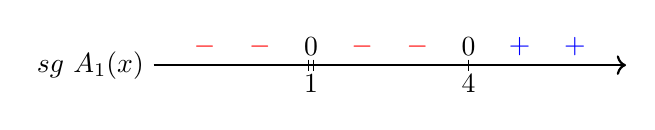
\begin{tikzpicture}
    % \draw[thin, opacity=1] (0, 0) -- (6, 0);
    \draw[thick,arrows=->] (0,0) -- (6,0);
    \foreach \x in {2}
      {
        \coordinate (A\x) at ($(0,0)+(\x+1.9cm,0)$) {};
        \draw ($(A\x)+(0,2pt)$) -- ($(A\x)-(0,2pt)$);
      }

    \foreach \x in {2}
      {
        \coordinate (A\x) at ($(0,0)+(\x+1.96cm,0)$) {};
        \draw ($(A\x)+(0,2pt)$) -- ($(A\x)-(0,2pt)$);
      }

    \foreach \x in {4}
      {
        \coordinate (A\x) at ($(0,0)+(\x,0)$) {};
        \draw ($(A\x)+(0,2pt)$) -- ($(A\x)-(0,2pt)$);
      }

    \node[left] at (0,0) {$sg \ {A}_1(x)$};

    \node[above, color=red] at (0.65, 0) (-) {\text\large$-$};
    \node[above, color=red] at (1.35, 0) (-) {\text\large$-$};


    % \node at (2, 0) (1) {"};  % corregir marca
    \node[above] at (2, 0) (1) {0};
    \node[below] at (2, 0) (1) {1};

    \node[above, color=red] at (2.65, 0) (-) {\text\large$-$};
    \node[above, color=red] at (3.35, 0) (-) {\text\large$-$};

    % \node at (4, 0) (1) {'};  % corregir marca
    \node[above] at (4, 0) (1) {0};
    \node[below] at (4, 0) (1) {4};

    \node[above,color=blue] at (4.65, 0) (+) {+};
    \node[above,color=blue] at (5.35, 0) (+) {+};

  \end{tikzpicture}
\end{center}

Es ${A}_1(x)=P(x)-P(1)<0$ en un entorno de $1$, con $x\neq1$ por lo que $P(x)$ presenta un máximo relativo en $x=1$ por definición. Para ${x}_0 = 3$:
$$
  {A}_3(x) = P(x)-P(3) = P(x)-16 = x^3-6x^2+9x
$$
Efectuando las sucesivas divisiones de ${A}_3(x)$ por $(x-3)$ obtenemos:
$$
  {A}_3(x) = P(x)-P(3) = (x-3)^2 x
$$
Por la misma argumentación, $P(x)$ presentará también extremo relativo en $x=3$ y al ser:

% \begin{center}
%    \begin{tikzpicture}
%          \draw[thick, opacity=1] (0, 0) -- (6, 0);

%          \node[left] at (0,0) {sg ${A}_1(x)$};

%          \node[above, color=red] at (0.65, 0) (-) {\text\large$-$};
%          \node[above, color=red] at (1.35, 0) (-) {\text\large$-$};


%          % \node at (2, 0) (1) {"};  % corregir marca
%          \node[above] at (2, 0) (1) {0};
%          \node[below] at (2, 0) (1) {0};

%          \node[above, color=blue] at (2.65, 0) (+) {\text\large$+$};
%          \node[above, color=blue] at (3.35, 0) (+) {\text\large$+$};

%          % \node at (4, 0) (1) {'};  % corregir marca
%          \node[above] at (4, 0) (1) {0};
%          \node[below] at (4, 0) (1) {3};

%          \node[above,color=blue] at (4.65, 0) (+) {+};
%          \node[above,color=blue] at (5.35, 0) (+) {+};


%    \end{tikzpicture}
% \begin{center}



% CORRECCIÓN DE SIGNO DE LA GRÁFICA
\begin{center}
  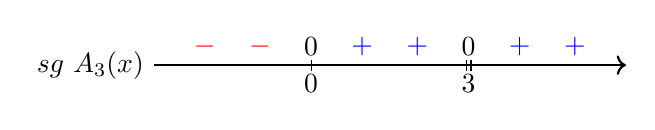
\begin{tikzpicture}
    % \draw[thin, opacity=1] (0, 0) -- (6, 0);
    \draw[thick,arrows=->] (0,0) -- (6,0);
    \foreach \x in {2}
      {
        \coordinate (A\x) at ($(0,0)+(\x,0)$) {};
        \draw ($(A\x)+(0,2pt)$) -- ($(A\x)-(0,2pt)$);
      }

    \foreach \x in {4}
      {
        \coordinate (A\x) at ($(0,0)+(\x+3.83cm,0)$) {};
        \draw ($(A\x)+(0,2pt)$) -- ($(A\x)-(0,2pt)$);
      }

    \foreach \x in {4}
      {
        \coordinate (A\x) at ($(0,0)+(\x+3.89cm,0)$) {};
        \draw ($(A\x)+(0,2pt)$) -- ($(A\x)-(0,2pt)$);
      }

    \node[left] at (0,0) {$sg \ {A}_3(x)$};

    \node[above, color=red] at (0.65, 0) (-) {\text\large$-$};
    \node[above, color=red] at (1.35, 0) (-) {\text\large$-$};


    % \node at (2, 0) (1) {"};  % corregir marca
    \node[above] at (2, 0) (1) {0};
    \node[below] at (2, 0) (1) {0};

    \node[above, color=blue] at (2.65, 0) (+) {\text\large$+$};
    \node[above, color=blue] at (3.35, 0) (+) {\text\large$+$};

    % \node at (4, 0) (1) {'};  % corregir marca
    \node[above] at (4, 0) (1) {0};
    \node[below] at (4, 0) (1) {3};

    \node[above,color=blue] at (4.65, 0) (+) {+};
    \node[above,color=blue] at (5.35, 0) (+) {+};

  \end{tikzpicture}
\end{center}

Es ${A}_3(x) = P(x)-P(3) > 0$ en un entorno de $3$, con $x\neq3$ por lo que $P(x)$ presenta un mínimo relativo en $x=3$.

La vinculación entre los extremos relativos de $P(x)$ en $x={x}_0$ y la presencia de raíces de orden par, para $A(x)$ en dicho punto, se formaliza en el siguiente:

\subsection{
  Formulación del Teorema 1
}
\addtocontents{toc}{
  \hspace{12pt}
  (Condición necesaria y suficiente de existencia de extremo relativo para una función polinómica)
}
% \lipsum[2]

"La condición necesaria y suficiente para que una función polinómica $y=P(x)$ admita un extremo relativo en el punto $x={x}_0$, es que ${x}_0$ sea una raíz múltiple de orden par del polinomio $A(x)=P(x)-P({x}_0)$." \\


\subsection*{Demostración:}
Si $P(x)$ admite un extremo relativo en $x={x}_0$, entonces $P(x)-P({x}_0)$ tiene signo constante en un entorno centrado en ${x}_0$, con $x \neq {x}_0$, por definición. \\
Definido $A(x)=P(x)-P({x}_0)$, se sigue que $A({x}_0)=P({x}_0)-P({x}_0)=0$ \\
Al cumplirse:
$$
  A({x}_0)=0
$$
$A(x)$ será divisible por $x-{x}_0$ (Teorema de Descartes) y es expresable:
$$
  A(x)=(x-{x}_0){Q}_1(x)
$$
La consideración ${Q}_1({x}_0) \neq 0$ implicaría que $A(x)$ no cambia de signo en $(x-{x}_0)$ y entraríamos en contradicción con la supuesta existencia de extremo relativo para $P(x)$ en dicho punto. \\
Se desprende entonces ${Q}_1({x}_0) = 0$. \\
Por la misma argumentación es expresable:
$$
  {Q}_1(x) = (x-{x}_0){Q}_2(x)
$$
Reemplazando ${Q}_1$ en la anterior expresión para $A(x)$:
$$
  A(x)=(x-{x}_0)^2{Q}_2(x)
$$
Si ${Q}_2({x}_0) \neq 0$ el teorema está probado. \\
En caso contrario será ${Q}_2({x}_0)=0$ y existirá un polinomio ${Q}_3(x)$ tal que:
$$
  {Q}_2(x) = (x-{x}_0){Q}_3(x)
$$
Pudiendo expresarse:
$$
  A(x)=(x-{x}_0)^3{Q}_3(x)
$$
La consideración ${Q}_3({x}_0) \neq 0$ nos reenvía a la incompatibilidad con la hipótesis de extremo relativo para $P(x)$ en $x={x}_0$. \\
Al ser ${Q}_3({x}_0)=0$, existirá un ${Q}_4(x)$ de modo que ${Q}_3(x)=(x-{x}_0){Q}_4(x)$ y entonces:
$$
  A(x)=(x-{x}_0)^4 {Q}_4(x)
$$
Si ${Q}_4({x}_0) \neq 0$ el teorema está probado, si no, se reitera el razonamiento hasta obtener:
$$
  A(x)=(x-{x}_0)^{2h}{Q}_{2h}(x)
$$
con $h \in N$, $h \geqslant 1$ y ${Q}_{2h}({x}_0) \neq 0$. \\
El número de pasos para obtener esta expresión es finito ya que está acotado por el propio grado de $A(x)$. \\
En efecto, de la última igualdad se desprende:
$$
  2h \leqslant gr \ A(x)
$$
Recíprocamente, si partimos ahora de la hipótesis de que $A(x)=P(x)-P({x}_0)$ admite raíz múltiple de orden par en $x={x}_0$, podemos escribir:
$$
  A(x)=(x-{x}_0)^{2h}Q(x)\text{, \ con\ \ }Q({x}_0) \neq 0
$$
$A(x)=P(x)-P({x}_0)$ tendrá signo constante en un entorno de ${x}_0$ y por definición, $P(x)$ presentará extremo en dicho punto, lo que completa la demostración.
\clearpage

Aplicaremos ahora sucesivamente el Teorema 1 en los casos concretos de polinomios de grados 2, 3 y 4. Estas aplicaciones además de revelar algunas propiedades relacionadas con el grado, nos permitirán en cada caso obtener una condición necesaria bajo la hipótesis de existencia de extremo. \\
Atendiendo a las conclusiones obtenidas se observarán patrones de comportamiento, que nos permitirán conjeturar y generalizarlas a polinomios de grado $n$. \\
Nótese que como consecuencia del Teorema 1, un polinomio de grado 1 no puede tener extremo relativo en ningún ${x}_0 \in R$. \\
En efecto, el correspondiente $A(x)=P(x)-P({x}_0)$ tendrá también grado 1 y cambiará de signo en ${x}_0$.

\subsection{
  Aplicación del Teorema 1
}
\addtocontents{toc}{
  \hspace{12pt}
  (Casos de grados 2, 3 y 4, condiciones necesarias, obtención de las coordenadas \\
  del extremo para el caso de grado 2 y clasificación del mismo según el coeficiente principal)
}

\subsection*{Grado 2:}
$$
  P(x)=ax^2+bx+c \text{, \ } a\neq0
$$
$P(x)$ presenta extremo relativo en $x={x}_0 \Leftrightarrow $ el polinomio
$A(x)=P(x)-P({x}_0)$ admite raíz múltiple de orden par en $x={x}_0$ (Teorema 1).\\
Como $gr \ A(x) = gr \ P(x) = 2$, solo puede ser raíz doble. \\
Esto es:
$$
  A(x)=a(x-{x}_0)^2 \ \ \ \ \ \ \ \text{\textcolor{red}{(i)}}
$$
Por otro lado se tiene:
$$
  % \begin{array}{c}
  %    A(x)=P(x)-P({x}_0)=ax^2+bx+c-(a{x}_0^2+b{x}_0+c)=a(x^2-{x}_0^2)+b(x-{x}_0)=\cdots \\
  %    \\
  %    \cdots=a(x+{x}_0)(x-{x}_0)+b(x-{x}_0)=(x-{x}_0)[a(x+{x}_0)+b]
  % \end{array}
  \begin{array}{lll}
    A(x)=P(x)-P({x}_0)              \\
    \\
    =ax^2+bx+c-(a{x}_0^2+b{x}_0+c)  \\
    \\
    =a(x^2-{x}_0^2)+b(x-{x}_0)      \\
    \\
    =a(x+{x}_0)(x-{x}_0)+b(x-{x}_0) \\
    \\
    =(x-{x}_0)[a(x+{x}_0)+b]
  \end{array}
$$
Esta factorización nos muestra que el cociente $Q(x)$ de dividir $A(x)$ por $(x-{x}_0)$ es: $a(x+{x}_0)+b=Q(x)$ \\
Pero considerando \textcolor{red}{(i)} para $A(x)$, también es $Q(x)=a(x-{x}_0)$ \\
En virtud de la unicidad del cociente y resto para la división entera de polinomios es:
$$
  Q(x)=a(x-{x}_0)=a(x+{x}_0)+b \ \ \forall \ \ x \in R
$$
Al ser $Q({x}_0)=0$, será asimismo $a({x}_0+{x}_0)+b=0 \ \Rightarrow \ 2a{x}_0+b=0$ \\
Entonces como consecuencia de que $P(x)=ax^2+bx+c$ admite un extremo relativo en $x={x}_0$ se desprende la condición (necesaria) de que el polinomio $S(x)=2ax+b$ admita raíz ${x}_0$.
\\[50pt]
En el caso particular de ser $gr \ P(x)=2 $, la condición anterior además de ser necesaria, es suficiente. \\
En efecto partiendo de la condición $S({x}_0)=0$, se tiene:
$$
  2a{x}_0+b=0 \Rightarrow a{x}_0+a{x}_0+b=0 \Rightarrow a({x}_0+{x}_0)+b=0
$$
por lo que ${x}_0$ resulta ser raíz del polinomio:
$$
  Q(x)=a({x}_0+x)+b
$$

Como $Q({x}_0)=0$, será divisible por $(x-{x}_0)$ y es expresable:
$$
  \begin{array}{lll}
    Q(x)=a(x-{x}_0)
    \Rightarrow
    A(x)=P(x)-P({x}_0)=(x-{x}_0)[a(x+{x}_0)+b] \\
    \\
    =(x-{x}_0)a(x-{x}_0)=a(x-{x}_0)^2
  \end{array}
$$
y por el mismo Teorema 1, $P(x)$ admitirá extremo en $x={x}_0$. \\
Las observaciones anteriores nos permiten obtener las coordenadas del extremo relativo de toda función polinómica de segundo grado. \\
Efectivamente, $P(x)$ admite extremo relativo en $x={x}_0 \Leftrightarrow S({x}_0)=0 \\ \Leftrightarrow 2a{x}_0+b=0 \Leftrightarrow x_0=\frac{-b}{2a}$ \\
Además $P({x}_0)=P(-\frac{b}{2a})=\frac{4ac-b^2}{4a}$, por lo que las coordenadas del extremo son:
$$
  {x}_0=-\frac{b}{2a}\text{, \ }{y}_0=\frac{4ac-b^2}{4a}
$$

Para clasificar dicho extremo analizaremos el signo de $A(x)=P(x)-P({x}_0)=a(x-{x}_0)^2$, y al ser $(x-{x}_0)^2 > 0 \ \ \forall \ \ x \neq {x}_0$, será $sg \ A(x)=sg \ a$ en un entorno de ${x}_0$, por lo que:

\begin{enumerate}
  \item Si $a>0 \Rightarrow P(x)-P({x}_0)>0 \ \ \forall \ \ x\neq {x}_0$ y habrá mínimo relativo en $x={x}_0$

  \item Si $a<0 \Rightarrow P(x)-P({x}_0)<0 \ \ \forall \ \ x\neq {x}_0$ y habrá máximo relativo en $x={x}_0$
\end{enumerate}
\text{ \\ }

\subsection*{Grado 3:}

$$
  P(x)=ax^3+bx^2+cx+d \text{, \ } a \neq 0
$$
$P(x)$ presenta extremo relativo en $x={x}_0 \ \Leftrightarrow \ A(x)=P(x)-P({x}_0)$ admite raíz múltiple de orden par en dicho punto (Teorema 1).\\
Como $gr \ P(x)=3$, sólo puede ser raíz doble. Esto es:
$$
  A(x)=(x-{x}_0)^2 Q(x)\text{ \ con \ }Q({x}_0)\neq0 \text{ \ y \ }gr \ Q(x)=1
$$
Por otro lado:
$$
  \begin{array}{lll}
    A(x)=P(x)-P({x}_0)=ax^3+bx^2+cx+d-(a{x}_0^3+b{x}_0^2+c{x}_0+d)  \\
    \\
    = a(x^3-{x}_0^3)+b(x^2-{x}_0^2)+c(x-{x}_0)                      \\
    \\
    = a(x-{x}_0)(x^2+{x}_0x+{x}_0^2)+b(x-{x}_0)(x+{x}_0)+c(x-{x}_0) \\
    \\
    =(x-{x}_0)[a(x^2+{x}_0x+{x}_0^2)+b(x+{x}_0)+c]
  \end{array}
$$
Tenemos así dos factorizaciones que corresponden a $A(x)$ y deben coincidir.
$$
  A(x)=(x-{x}_0)^2 Q(x)=a(x-{x}_0)[a(x^2+{x}_0x+{x}_0^2)+b(x+{x}_0)+c]\text{, \ }\forall x \in R
$$
por lo que el cociente (único) de dividir $A(x)$ por $x-{x}_0$ admitirá también dos formas asimismo coincidentes.
$$
  (x-{x}_0)Q(x)=a(x^2+{x}_0x+{x}_0^2)+b(x+{x}_0)+c\text{, \ }\forall x \in R
$$
Como el miembro izquierdo admite manifiestamente la raíz $x={x}_0$, también la admitirá el miembro derecho, cumpliéndose que:
$$
  a({x}_0^2+{x}_0{x}_0+{x}_0^2)+b({x}_0+{x}_0)+c =0
$$
\begin{center}
  o bien:
\end{center}
$$
  3a{x}_0^2+2b{x}_0+c=0
$$
${x}_0$ resulta ser raíz del polinomio:
$$
  S(x)=3ax^2+2bx+c
$$
Una condición necesaria de suponer que $P(x)$ presenta extremo relativo en $x={x}_0$.
\\

\subsection*{Grado 4:}
$$
  P(x)=ax^4+bx^3+cx^2+dx+e \text{, \ } a \neq 0
$$
$P(x)$ presenta extremo relativo en $x={x}_0 \ \Leftrightarrow \ A(x)=P(x)-P({x}_0)$ admite raíz múltiple ${x}_0$ de orden par en dicho punto (Teorema 1).\\
Las opciones son:
\begin{enumerate}
  \item $A(x)=(x-{x}_0)^2 Q(x)$, \ con \ $Q({x}_0)\neq0$ \ y \ $gr \ Q(x)=2$

  \item $A(x)=a(x-{x}_0)^4$
\end{enumerate}

Considerando el caso n°1, tendremos:
$$
  \begin{array}{lll}
    A(x)=P(x)-P({x}_0)=ax^4+bx^3+cx^2+dx+e-(a{x}_0^4+b{x}_0^3+c{x}_0^2+d{x}_0+e) \\
    \\
    =a(x^4-{x}_0^4)+b(x^3-{x}_0^3)+c(x-{x}_0^2)+d(x-{x}_0)                       \\
    \\
    =a(x-{x}_0)(x^3+{x}_0x^2+{x}_0^2x+{x}_0^3)+b(x-{x}_0)(x^2+{x}_0x+{x}_0^2)    \\
    +c(x-{x}_0)(x+{x}_0)+d(x-{x}_0)                                              \\
    \\
    =(x-{x}_0)[a(x^3+{x}_0x^2+{x}_0^2x+{x}_0^3)+b(x^2+{x}_0x+{x}_0^2)+c(x+{x}_0)+d]
  \end{array}
$$
Como en los casos anteriores al considerar la división de $A(x)$ por $x-{x}_0$ se tiene por el caso n°1, que el cociente es $(x-{x}_0)Q(x)$ y también la expresión polinómica entre paréntesis rectos. \\
Por la referida unicidad del cociente y considerando que $(x-{x}_0)Q(x)$ admite manifiestamente raíz ${x}_0$, asimismo ocurrirá con la expresión entre paréntesis rectos, cumpliéndose:
$$
  a({x}_0^3+{x}_0^3+{x}_0^3+{x}_0^3)+b({x}_0^2+{x}_0^2+{x}_0^2)+c({x}_0+{x}_0)+d=0
$$
\begin{center}
  o bien:
\end{center}
$$
  4a{x}_0^3+3b{x}_0^2+2c{x}_0+d=0
$$

${x}_0$ resulta ser raíz del polinomio:
$$
  S(x)=4ax^3+3bx^2+2cx+d
$$
Una condición necesaria de suponer que $P(x)$ admite extremo relativo en $x={x}_0$.

Considerando el caso n°2, tendremos:
$$
  A(x)=a(x-{x}_0)^4=(x-{x}_0)^2a(x-{x}_0)^2
$$
Designando con $K(x)$, se sigue que:
$$
  A(x)=(x-{x}_0^2)K(x)
$$
Pudiendo adoptar $A(x)$ una estructura análoga al caso n°1 nos conducirá al mismo resultado:
$$
  S({x}_0)=0
$$
La única diferencia radica en que $K({x}_0)=0$ mientras que $Q({x}_0)\neq0$. \\
Sin embargo el razonamiento efectuado en el caso n°1 será válido toda vez que $A(x)$ admita al menos dos raíces iguales a ${x}_0$. \\


\subsection{
  Recopilación de las condiciones necesarias en los casos estudiados, identificación de patrones y definición de sub-polinomio
}

Haremos ahora una pausa momentánea para ordenar los resultados obtenidos hasta el momento, en forma de tabla, donde figurará cada polinomio $S(x)$, asociado a su respectivo $P(x)$.
\textcolor{red}{
  \begin{center}
    \begin{tabular}{ |c|c|c| }
      \hline
      \textbf{\textcolor{black}{P(x)}}         & \textbf{\textcolor{black}{S(x)}}       \\
      \hline
      \textcolor{black}{$ax^2+bx+c$}           & \textcolor{black}{$2ax+b$}             \\
      \hline
      \textcolor{black}{$ax^3+bx^2+cx+d$}      & \textcolor{black}{$3ax^2+2bx+c$}       \\
      \hline
      \textcolor{black}{$ax^4+bx^3+cx^2+dx+e$} & \textcolor{black}{$4ax^3+3bx^2+2cx+d$} \\
      \hline
    \end{tabular}
  \end{center}
}

% TABLA ORIGINAL SIN CAMBIO DE COLOR
% \begin{center}
% \begin{tabular}{ |c|c|c| } 
% \hline
% \textbf{P(x)} & \textbf{S(x)} \\ 
% \hline
% $ax^2+bx+c$ & $2ax+b$ \\ 
% \hline
% $ax^3+bx^2+cx+d$ & $3ax^2+2bx+c$ \\ 
% \hline
% $ax^4+bx^3+cx^2+dx+e$ & $4ax^3+3bx^2+2cx+d$ \\
% \hline
% \end{tabular}
% \end{center}

La contemplación de la tabla sugiere claros patrones en la determinación de $S(x)$ a partir de su correspondiente $P(x)$. \\
Para transformar cada término de $ $ en su respectivo de $S(x)$, basta multiplicarlo por su grado y disminuir este último en una unidad; prescindiendo de su término independiente.

En forma genérica la correspondencia observada puede representarse:
$$
  \text{\Large$
      ax^n \rightarrow nax^{n-1} \ \ \ \ n \geqslant 1
    $}
$$
Atendiendo a estas observaciones daremos la siguiente:

\subsection*{Definición:}
Dada una función polinómica $P:R \rightarrow R$
$$
  P(x)={a}_n x^n+{a}_{n-1} x^{n-1}+\cdots+{a}_1 x+{a}_0\text{, \ }n\geqslant1\text{, \ }{a}_n\neq0
$$
llamaremos sub-polinomio $S(x)$ asociado a $P(x)$ al siguiente:
$$
  S(x)=n{a}_{n}x^{n-1}+(n-1){a}_{n-1}x^{n-2}+\cdots+2{a}_2x+{a}_1
$$
Cuando se quiera enfatizar esta asociación se indicará con la notación ${S}_P(x)$.

De acuerdo a esta definición cada polinomio de grado $n\geqslant1$ tendrá asociado un único polinomio $S(x)$ de grado $n-1$ siendo $S(x)$ independiente de ${a}_0$. \\
(Si P(x) tuviese grado cero, sería $P(x)={a}_0$. En este caso definimos ${S}_P(x)\equiv0$).\\
Esta independencia se formaliza en el siguiente: \\

\subsection{Teorema 2}
\addtocontents{toc}{
\hspace{12pt}
(Condición necesaria y suficiente para que dos polinomios $A(x)$ y $B(x)$ tengan el \\
mismo sub-polinomio $S(x)$)
}
La condición necesaria y suficiente para que dos polinomios $A(x)$ y $B(x)$ tengan el mismo sub-polinomio $S(x)$ es que dichos polinomios difieran en una constante.

Demostración:

Sean en efecto dos polinomios $A(x)$ y $B(x)$ que supondremos de grado no nulo. \\
Si tienen el mismo sub-polinomio $S(x)$ entonces por definición será:

$$
  \begin{array}{ccc}
    gr \ S(x)= gr \ A(x)-1 \\
    \\
    gr \ S(x)= gr \ B(x)-1
  \end{array}
$$

\begin{center}
  por lo que resulta:
\end{center}
$$
  gr \ A(x)=gr \ B(x)
$$

Pongamos:

$$
  \begin{array}{ccc}
    A(x)={a}_n x^n+{a}_{n-1} x^{n-1}+\cdots+{a}_1 x+{a}_0 \\
    \\
    B(x)={b}_n x^n+{b}_{n-1} x^{n-1}+\cdots+{b}_1 x+{b}_0 \\
    \\
    S(x)={s}_{n-1} x^{n-1}+\cdots+{s}_1 x+{s}_0
  \end{array}
$$

Se tiene por definición:

$$
  \begin{aligned}
    \left\{
    \begin{array}{ccc}
      {s}_{n-1}=n{a}_n \\
      \\
      {s}_{n-1}=n{b}_n
    \end{array}
    \right.
     &
    \Rightarrow {a}_n = {b}_n
     &   &  &
    \left\{
    \begin{array}{ccc}
      {s}_{n-2}=(n-1){a}_{n-1} \\
      \\
      {s}_{n-2}=(n-1){b}_{n-1}
    \end{array}
    \right.
     &
    \Rightarrow {a}_{n-1} = {b}_{n-1}
  \end{aligned}
$$

y en general se tendrá ${a}_i={b}_i$ con $i=1,2,\cdots,n$ por lo que al considerar la diferencia: \\
$$
  A(x)-B(x)=({a}_n - {b}_n)x^n + ({a}_{n-1} - {b}_{n-1})x^{n-1} +\cdots+ ({a}_1-{b}_1)x+{a}_0-{b}_0
$$
serán nulos todos los coeficientes de $x^i$, con $i=1,\cdots,n$ y entonces $A(x)-B(x)={a}_0-{b}_0$ que es constante para todo $x$.

Si partimos recíprocamente de $A(x)-B(x)=k$ para todo $x$ real, con $k$ constante, se tiene:
$$
  A(x)=B(x)+k
$$
En virtud del Teorema de Identidad de Polinomios se deduce que ${a}_i={b}_i$ para $i=1,2,\cdots,n$ .\\
Los respectivos sub-polinomios asociados a $A(x)$ y $B(x)$ son:
$$
  \begin{array}{ccc}
    {S}_A (x)=n{a}_n x^{n-1}+(n-1){a}_{n-1}x^{n-2}+\cdots+2{a}_2 x+{a}_1 \\
    \\
    {S}_B (x)=n{b}_n x^{n-1}+(n-1){b}_{n-1}x^{n-2}+\cdots+2{b}_2 x+{b}_1
  \end{array}
$$

Al cumplirse ${a}_i={b}_i$ con $i=1,2,\dots,n$ será asimismo $i{a}_i=i{b}_i$ con $i=1,2,\dots,n$ y en consecuencia será:
$$
  \text{\Large ${S}_A (x)={S}_B (x)$}
$$
como se quería probar.


\subsection{
  Teorema 3
}
\addtocontents{toc}{
  \hspace{12pt}
  (Propiedades de linealidad de los sub-polinomios)
}
\begin{enumerate}
  \item El sub-polinomio asociado al polinomio suma $(A+B)(x)$, es igual a la suma de los sub-polinomios asociados a cada uno de los sumandos $A(x)$ y $B(x)$. \\
        Esto es:
        $$
          {S}_{A+B}(x)={S}_A(x)+{S}_B(x)
        $$

  \item Si un polinomio se multiplica por una constante su sub-polinomio queda multiplicado por dicha constante:
        $$
          {S}_{K(p)}(x)=K{S}_P(x)
        $$
\end{enumerate}

Haremos la demostración de la primera siendo la segunda más sencilla y evidente.

\subsection*{Demostración:}
Sean $A(x)$ y $B(x)$ dos polinomios de grados $m$ y $n$ respectivamente con $m \geqslant n \geqslant 1$.
$$
  \begin{array}{ccc}
    A(x)={a}_m x^m + {a}_{m-1}x^m-1 + \cdots + {a}_{n+1} x^{n+1} + {a}_n x^n + {a}_{n-1} x^{n-1} + \cdots + {a}_1 x + {a}_0                                                    \\
    \\
    B(x)= \ \ \ \ \ \ \ \ \ \ \ \ \ \ \ \ \ \ \ \ \ \ \ \ \ \ \ \ \ \ \ \ \ \ \ \ \ \ \ \ \ \ \ \ \ \ \ \ \ \ \ \ \ \ {b}_n x^n + {b}_{n-1} x^{n-1} + \cdots + {b}_1 x + {b}_0 \\
    \\
    (A+B)(x)={a}_m x^m + {a}_{m-1}x^m-1 + \cdots + {a}_{n+1} x^{n+1} + ({a}_n+{b}_n) x^n +\cdots+ ({a}_1+{b}_1)x+{a}_0+{b}_0
  \end{array}
$$

Por definición es:
$$
  \begin{array}{ccc}
    {S}_{A+B}(x)=m{a}_m x^{m-1}+\cdots+(n+1){a}_{n+1} x^n + n({a}_n+{b}_n)x^{n-1} +\cdots+ {a}_1+{b}_1 \\
    \\
    \text{Haciendo distributiva y reordenando términos:}                                               \\
    \\
    {S}_{A+B}(x)=m{a}_m x^{m-1}+\cdots+(n+1){a}_{n+1} x^n + n{a}_n x^{n-1}+\cdots+2{a}_2 x+{a}_1+      \\
    \\
    n{b}_n x^{n-1}+\cdots+2{b}_2 x+{b}_1=                                                              \\
    \\
    \text{\Large ${S}_A (x) + {S}_B (x)$}
  \end{array}
$$

%resultado con \text{\Large $ $}



\subsection{
  Teorema 4
}
\addtocontents{toc}{
\hspace{12pt}
(La imagen de ${x}_0$ a través de ${S}_P$, sub-polinomio de $P(x)$, coincide con la imagen de ${x}_0$ a través de $H(x)$, cociente de dividir $P(x)-P({x}_0)$ por $x - {x}_0$)
}
Sea $P(x)$ una función polinómica $P:R \rightarrow R$ con $gr \ P(x) \geqslant 2$, \ ${x}_0 \in R$.
$$
  A(x)=P(x)-P({x}_0)
$$
${S}_P(x)$ es el sub-polinomio asociado a $P(x)$. \\
Entonces:
\begin{enumerate}[i)]
  \item Existe un polinomio $H(x)$, con $gr \ H(x) \geqslant 1$ tal que $A(x)=(x-{x}_0)H(x)$

  \item $H({x}_0)={S}_P({x}_0)$
\end{enumerate}

\subsection*{Demostración:}
Como $A({x}_0)=P({x}_0)-P({x}_0)=0$, $A(x)$ es divisible por $x-{x}_0$ por lo que existe $H(x)$ tal que:
$$
  A(x)=(x-{x}_0){H(x)}_{\textcolor{red}{(*)}}
$$
con $gr \ H(x)=gr \ A(x)-1=gr \ P(x)-1$, y al ser $gr \ P(x) \geqslant 2$, es $gr \ P(x)-1 \geqslant 1 \Rightarrow gr \ H(x) \geqslant 1$

Por otro lado es:
$$
  \begin{array}{lll}
    P(x)-P({x}_0)={a}_n x^n+{a}_{n-1} x^{n-1}+\cdots+{a}_1 x+{a}_0-({a}_n {x}_0^n+{a}_{n-1} {x}_0^{n-1}+\cdots+{a}_1{x}_0+{a}_0)= \\
    \\
    {a}_n(x^n-{x}_0^n)+{a}_{n-1}(x^{n-1}-{x}_0^{n-1})+\cdots+{a}_2(x^2-{x}_0^2)+{a}_1(x-{x}_0)=                                   \\
    \\
    {a}_n(x-{x}_0)(x^{n-1}+{x}_0 x^{n-2}+\cdots+{x}_0^{n-1})+\cdots+{a}_2(x-{x}_0)(x+{x}_0)+{a}_1(x-{x}_0)=                       \\
    \\
    (x-{x}_0)[{a}_n(x^{n-1}+{x}_0 x^{n-2}+\cdots+{x}_0^{n-1})+\cdots+{a}_2(x+{x}_0)+{a}_1]={A(x)}_{\textcolor{red}{(**)}}
  \end{array}
$$


Observando las expresiones \textcolor{red}{(*)} y \textcolor{red}{(**)} para $A(x)$ tenemos que tanto $H(x)$ como la expresión entre paréntesis rectos, son el cociente de dividir $A(x)$ por $(x-{x}_0)$ que en virtud de la unicidad del mismo deben coincidir, por lo que:
$$
  \begin{array}{ccc}
    H({x}_0)={a}_n({x}_0^{n-1}+{x}_0^{n-1}+\cdots+{x}_0^{n-1})+\cdots+{a}_2({x}_0+{x}_0)+{a}_1= \\
    \\
    n{a}_n {x}_0^{n-1}+\cdots+2{a}_2 {x}_0+{a}_1= {S}_P({x}_0)
  \end{array}
$$

Este teorema nos dice que la imagen de ${x}_0$ a través de $H(x)$, cociente de dividir $A(x)=P(x)-P({x}_0)$ por $(x-{x}_0)$, coincide con la imagen de ${x}_0$ a través del sub-polinomio ${S}_P(x)$, asociado a $P(x)$.

\subsection{
  Teorema 5
}
\addtocontents{toc}{
\hspace{12pt}
(Lema del sub-polinomio, si $P(x)=(x-{x}_0)^2.Q(x)$ entonces ${x}_0$ es raíz de su sub-polinomio ${S}_P(x)$)
}
% \begin{center}
"Si un polinomio $P(x)$ admite una factorización de la forma:
$P(x)=(x-{x}_0)^2 N(x)$
entonces, ${x}_0$ es raíz de su sub-polinomio ${S}_P(x)$.
Esto es:
$$
  {S}_P({x}_0)=0\text{"}
$$
% \end{center}

\subsection*{Demostración:}
Consideremos $A(x)=P(x)-P({x}_0)$. Al ser $P(x)=(x-{x}_0)^2 N(x)$, es $gr \ P(x) \geqslant 2$ y estamos en las hipótesis del Teorema 4. \\
\begin{center}
  Existe un polinomio $H(x)$ tal que:
  $$
    A(x)=P(x)-P({x}_0)=(x-{x}_0)H(x)
  $$
  con la condición: $H({x}_0)={S}_P({x}_0)$ \\
  Por otro lado $P({x}_0)=({x}_0-{x}_0)^2 N({x}_0)=0$ y entonces:
  $$
    A(x) \equiv P(x)=(x-{x}_0)^2 N(x)=(x-{x}_0)(x-{x}_0)N(x)
  $$
\end{center}
Al cumplirse $A(x)=(x-{x}_0)H(x)$, resulta $(x-{x}_0)N(x)=H(x)$, por lo que $H({x}_0)=0$, pero siendo $H({x}_0)={S}_P ({x}_0)$, se obtiene:
$$
  \text{\Large{${S}_P({x}_0)=0$}}
$$

\subsection{
  Teorema 6
}
\addtocontents{toc}{
  \hspace{12pt}
  (Aplicación del Lema, condición necesaria de existencia de extremo para una función polinómica)
}
"Si una función polinómica $P:R \rightarrow R$, con $gr \ P(x) \geqslant 2$, presenta un extremo relativo en $x={x}_0$, entonces ${x}_0$ es raíz de su sub-polinomio ${S}_P(x)$"

\subsection*{Demostración:}
$P(x)$ presenta extremo relativo en $x={x}_0$ por hipótesis. Por Teorema 1, $A(x)=P(x)-P({x}_0)$ admite raíz múltiple de ${x}_0$, de orden par. \\
Esto es: $A(x)=(x-{x}_0)^{2k}Q(x)$, con $k \in N $, \ $k \geqslant 1$. \\
Poniendo $A(x)=(x-{x}_0)^2(x-{x}_0)^{2k-2}Q(x)$ y designando $N(x)=(x-{x}_0)^{2k-2}Q(x)$, es:
$$
  A(x)=(x-{x}_0)^2 N(x)
$$
Aplicando el Teorema 5, ${x}_0$ será raíz de ${S}_A(x)$, es decir ${S}_A({x}_0)=0$. \\
De $A(x)=P(x)-P({x}_0)$ se obtiene $P(x)-A(x)=P({x}_0)$, que muestra que $P(x)$ y $A(x)$ difieren en una constante, y entonces por Teorema 2 tendrán el mismo sub-polinomio. Esto es:
$$
  {S}_P(x)={S}_A(x) \ \ \forall \ \ x \in R
$$
\begin{center}
  Haciendo $x={x}_0$, \ ${S}_P({x}_0)={S}_A({x}_0)=0$, es decir:
\end{center}
$$
  \text{\Large{${S}_P({x}_0)=0$}}
$$
como se quería probar.
\clearpage

Hasta el momento hemos hablado de condiciones necesarias de existencia de extremo, por un lado, valiéndonos de los sub-polinomios.\\
Las raíces de estos nos proporcionan los "candidatos" a extremo relativo, es decir, los puntos factibles donde estos extremos podrían alcanzarse.\\
Como criterio de clasificación disponemos de la condición necesaria y suficiente aportada por el Teorema 1.\\
El polinomio $A(x)=P(x)-P({x}_0)$ debe admitir raíz múltiple de orden par en $x={x}_0$ para asegurar la existencia de extremo. Para clasificar dicho extremo hará falta conocer el signo de $A(x)$ en un entorno de ${x}_0$ y frecuentemente conocer sus raíces, tarea que resultará más ardua y costosa a medida que aumenta el grado de $A(x)$ ($gr \ A(x)=gr \ P(x)$).\\
Daremos a continuación un criterio que nos permitirá decidir si en $x={x}_0$ (raíz de ${S}_P(x)$) la función polinómica presenta un máximo o un mínimo relativo, o no tiene extremo, sin necesidad de hallar otras raíces de $A(x)$, aparte de ${x}_0$.\\
Previamente necesitaremos probar un teorema, similar al Teorema de conservación del signo para funciones Reales pero dirigido exclusivamente a polinomios, cuya fundamentación "elemental" será viable en el caso de que estos tengan raíces.\\
De todas formas existen numerosas situaciones en las que es posible probar que un polinomio tiene signo constante aunque no tenga raíces.\\
Dado que estamos desarrollando una Teoría elemental no pretendemos abordar con ella todos los resultados obtenidos por el Cálculo para funciones Reales en general. La idea es dar un indicio, un primer acercamiento teórico en circunstancias favorables, que permita enunciar reglas de acción fundamentadas.
\clearpage

\subsection{
  Teorema 7
}
\addtocontents{toc}{
  \hspace{12pt}
  (De "conservación" del signo, para polinomios con raíces reales)
}
Sea una función polinómica $P:R \rightarrow R$, de grado $n \geqslant 2$, con $n$ raíces distintas:
$$
  \begin{array}{ccc}
    {\alpha}_1 < {\alpha}_2 < \cdots < {\alpha}_n \\
    \\
    {x}_0 \in R \text{ \ y \ } P({x}_0) \neq 0
  \end{array}
$$
Entonces es posible encontrar un entorno centrado en ${x}_0$ de modo que $sg \ P(x)=sg \ P({x}_0)$ para todos los $x$ de dicho entorno.\\
Esto es, existe un $r > 0$ tal que $\forall \ x \in {E}_{{x}_0, r}$ es $P(x)>0$ \ ó \ $P(x)<0$.

\subsection*{Demostración:}
\begin{center}
  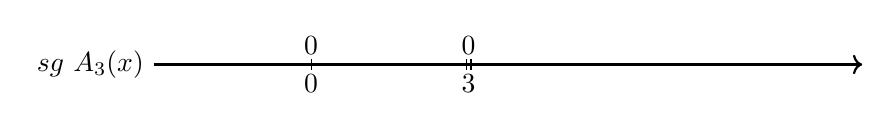
\begin{tikzpicture}
    % \draw[thin, opacity=1] (0, 0) -- (6, 0);
    \draw[thick,arrows=->] (0,0) -- (9,0);
    \foreach \x in {2}
      {
        \coordinate (A\x) at ($(0,0)+(\x,0)$) {};
        \draw ($(A\x)+(0,2pt)$) -- ($(A\x)-(0,2pt)$);
      }

    \foreach \x in {4}
      {
        \coordinate (A\x) at ($(0,0)+(\x+3.83cm,0)$) {};
        \draw ($(A\x)+(0,2pt)$) -- ($(A\x)-(0,2pt)$);
      }

    \foreach \x in {4}
      {
        \coordinate (A\x) at ($(0,0)+(\x+3.89cm,0)$) {};
        \draw ($(A\x)+(0,2pt)$) -- ($(A\x)-(0,2pt)$);
      }

    \node[left] at (0,0) {$sg \ {A}_3(x)$};

    % signos de menos
    % \node[above, color=red] at (0.65, 0) (-) {\text\large$-$};
    % \node[above, color=red] at (1.35, 0) (-) {\text\large$-$};


    % \node at (2, 0) (1) {"};  % corregir marca
    \node[above] at (2, 0) (1) {0};
    \node[below] at (2, 0) (1) {0};

    % signos de mas
    % \node[above, color=blue] at (2.65, 0) (+) {\text\large$+$};
    % \node[above, color=blue] at (3.35, 0) (+) {\text\large$+$};

    % \node at (4, 0) (1) {'};  % corregir marca
    \node[above] at (4, 0) (1) {0};
    \node[below] at (4, 0) (1) {3};

    % signos de mas
    % \node[above,color=blue] at (4.65, 0) (+) {+};
    % \node[above,color=blue] at (5.35, 0) (+) {+};

  \end{tikzpicture}
\end{center}

Consideremos el $sg \ P(x)$ según la ilustración precedente. Como consecuencia del Teorema de descomposición factorial, $P(x)$ no puede cambiar de signo entre dos raíces consecutivas, a la derecha de la mayor ${\alpha}_n$, ni a la izquierda de la menor ${\alpha}_1$. \\
En los tres casos basta tomar como radio del entorno, la distancia de ${x}_0$ a "la más cercana" de las raíces.\\
Esto es:
$$
  r=min \{|{x}_0-{\alpha}_i|, \ i=1,2,\cdots,n, \ P({\alpha}_i)=0\}
$$
y entonces $sg \ P(x)=sg \ P({x}_0) \ \forall \ x \in {E}_{{x}_0, r}$

Observación:\\
A pesar de que en la hipótesis hemos admitido $ $ raíces distintas, es fácil contemplar otros casos de raíces múltiples donde figurarán factores del tipo $(x-\alpha)^h$ en la descomposición factorial o incluso factores polinómicos de signo constante.

\subsection{
  Teorema 8
}
\addtocontents{toc}{
  \hspace{12pt}
  (Condiciones suficientes, Criterios de clasificación de presuntos extremos relativos)
}
$P(x)$ es una función polinómica $P:R \rightarrow R$,\  con \ $gr \ P \geqslant 2$.\\
${S}_P$ es su sub-polinomio asociado, ${x}_0 \in R$ \ con \ ${S}_P({x}_0)=0$. \ $A(x)=P(x)-P({x}_0)$ \\
Entonces: \\

\begin{enumerate}[i)]
  \item Existen $\lambda \in N$, $\lambda \geqslant 2$ y $Q:R \rightarrow R$, función polinómica, de modo que $A(x)=(x-{x}_0)^\lambda Q(x)$ y $Q({x}_0) \neq 0$.

  \item Si $\lambda$ es impar, $P(x)$ no presenta extremo en $x={x}_0$.

  \item Si $\lambda$ es par, $P(x)$ presenta extremo relativo en $x={x}_0$ y es:
        \begin{itemize}
          \item máximo relativo si $Q({x}_0)<0$
        \end{itemize}
        \ \ \ \ ó
        \begin{itemize}
          \item mínimo relativo si $Q({x}_0)>0$
        \end{itemize}
\end{enumerate}

\subsection*{Demostración:}
\begin{enumerate}[i)]
  \item Como $A({x}_0)=P({x}_0)-P({x}_0)=0$, $A(x)$ es divisible por $(x-{x}_0)$, por lo que existe un polinomio $H(x)$ que cumple:
        $$
          A(x)=(x-{x}_0)H(x)
        $$

        Empleando el Teorema 4 se tiene: \\
        $H({x}_0)=0$ y por hipótesis es ${S}_P({x}_0)=0$ por lo que $H({x}_0)=0$. De aquí, $H(x)$ es divisible por $(x-{x}_0)$ y existirá un $Q(x)$, tal que:
        $$
          H(x)=(x-{x}_0)Q(x)
        $$
        Reemplazando $H(x)$ en la expresión factorizada de $A(x)$:
        $$
          A(x)=(x-{x}_0)(x-{x}_0)Q(x)=(x-{x}_0)^2 Q(x)
        $$

        Si $Q({x}_0) \neq 0$, está probada la parte i). \\
        En caso contrario ${x}_0$ será raíz de orden $h$ de $Q(x)$ y podrá expresarse:
        $$
          Q(x)=(x-{x}_0)^h {Q}_1(x) \text{, \ con \ } {Q}_1({x}_0) \neq 0 \text{ \ y \ } h \geqslant 1
        $$

        Reemplazando en la última expresión para $ $, se obtiene:
        $$
          x
        $$
        tomando $ $, como $ $ también queda probada la parte i).

  \item Considerando $ $ con $ $ siendo $ $, si $ $ es impar, por el Teorema 1, $ $ no puede tener extremo relativo en $ $.

  \item Si $ $ es par, por el mismo Teorema 1, $ $ presenta extremo relativo en $ $. \\
        $ $ y $  \  $. \\
        Si $ $, por Teorema 7 existe un entorno centrado en $ $ de modo que:
        $$
          x
        $$
        Por lo que será $ $. \\
        $ $ tendrá un máximo relativo en $ $, por definición.\\
        Si $ $, por Teorema 7, existe un $ $ tal que:
        $$
          x
        $$
        por lo que será $ $.\\
        $ $ tendrá un mínimo relativo en $ $, por definición.

\end{enumerate}

\subsection{
  Recopilación de procedimientos prácticos para identificar y clasificar extremos, ejemplos diversos resueltos
}
\section*{\ul{Pausa práctica:}}
Para darle un sentido práctico al estudio realizado hasta el momento, resumimos un conjunto de pasos a seguir para la determinación de presuntos extremos y su posterior clasificación empleando la teoría expuesta.

\begin{enumerate}
  \item Calculamos el sub-polinomio asociado a $ $, cuyos extremos relativos se buscan y resolvemos la ecuación $ $ (condición necesaria).

  \item Para cada $ $ raíz de la ecuación anterior consideramos el polinomio $ $ y efectuamos las sucesivas divisiones por $ $, hasta obtener:
        $$
          x
        $$

  \item Si $ $ es impar, no hay extremo relativo en $ $.

  \item Si $ $ es par (condición necesaria y suficiente), existe extremo en $ $, cumpliéndose:
        \begin{itemize}
          \item Máximo relativo si $ $
        \end{itemize}
        \ \ \ \ ó
        \begin{itemize}
          \item Máximo relativo si $ $.
        \end{itemize}
\end{enumerate}

\section*{\ul{Ejemplos diversos}}
\begin{enumerate}
  \item Determinar si existen los extremos relativos de $ $.

        \subsection*{Resolución:}
        $$
          \begin{array}{ccc}
            x \\
            \\
            x \ \text{(condición necesaria)}
          \end{array}
        $$
        La ecuación $ $ tiene raíz doble: $ $, único candidato a extremo en este caso.\\
        Como $ $.\\
        Al efectuar las sucesivas divisiones por $ $, se obtiene:
        $$
          g
        $$
        al ser $ $ impar, $ $ no presenta extremo en $ $.

  \item Determinar si existen los extremos relativos de $ $.

        \subsection*{Resolución:}
        $$
          \begin{array}{ccc}
            x \\
            \\
            x \ \text{(condición necesaria)}
          \end{array}
        $$
        La ecuación $ $ tiene raíz evidente $ $. Al efectuar la correspondiente división, se obtiene:
        $$
          c
        $$
        por lo que $ $ resulta ser la única raíz Real.\\
        Como $ $.\\
        Efectuando las correspondientes divisiones sucesivas de $ $ por $ $, se obtiene:
        $$
          f
        $$
        En este caso $ $, par, por lo que $ $ presenta extremo en $ $, además $ $.\\
        Al ser $ $, se trata de un mínimo relativo en $ $.

        \subsection*{Observación:}
        En el caso precedente $ $ no tiene raíces Reales y no estamos en las hipótesis del Teorema 7.\\
        Sin embargo $ $ es manifiestamente positivo al ser $ $, y se cumple que existe un entorno de 1, de modo que $ $.\\
        No asumiremos el compromiso de demostrar el Teorema 7 en el caso de no haber raíces Reales para $ $, para no apartarnos del enfoque elemental que caracteriza la presente Teoría.\\
        Con argumentos similares al aquí empleado, se pueden clasificar los presuntos extremos de una función polinómica, "extendiendo" el Teorema 7 (de conservación del signo) probando que $ $ tiene signo constante aunque no tenga raíces Reales.

  \item Determinar si existen los extremos relativos de $ $.

        \subsection*{Resolución:}
        $$
          \begin{array}{ccc}
            x \\
            \\
            x \ \text{(condición necesaria)}
          \end{array}
        $$
        Las raíces de la ecuación $ $ son: \{1,3,4\}

        Para $ $:
        $$
          x
        $$
        Efectuando las sucesivas divisiones de $ $ por $ $, hasta encontrar un resto no nulo, obtenemos:
        $$
          x
        $$
        $ $, y $ $, como $ $ es par hay extremo en $ $ y al no tener raíces Reales la ecuación $ $, $ $ tendrá signo constantemente positivo. Siguiendo los pasos prácticos recopilados, igual se cumple que $ $ y se concluye que $ $ presenta un mínimo en $ $.

        Para $ $:
        $$
          x
        $$
        Efectuando las sucesivas divisiones de $ $ por $ $ obtenemos:
        $$
          \begin{array}{ccc}
            x \\
            \\
            \text{con \ } x \text{ \ y } x
          \end{array}
        $$

        Al ser $ $ par, hay extremo en $ $. En este caso la ecuación $ $ tiene raíces Reales, es aplicable el Teorema 7, al ser $ $, \ $ $ presenta un máximo relativo en $ $.

        Para $ $:
        $$
          x
        $$
        Aquí, $ $ es par y $ $, por lo que $ $ tendrá un mínimo relativo en $ $.
\end{enumerate}

\subsection{
  \ul{Figura de análisis y definición elemental de recta tangente al gráfico de $y=P(x)$ en un punto $({x}_0,{y}_0)$ de la curva}
}

\begin{center}
  \begin{tikzpicture}
    \begin{axis}[
        standard,
        clip=false,
        xmin=0, xmax=6, ymin=0, ymax=1.3, axis lines=left,
        xlabel=$x$,
        ylabel=$y$,
        xtick={2.18, 3},
        xticklabels={$x$, ${x}_0$},
        ytick={0.2, 0.6},
        yticklabels={$P({x}_0)$, $P(x)$},
        % yticklable style={anchor=east}
      ]

      \addplot[
        color=blue,
        % fill=red,
        % fill opacity=0.2,
        samples=200,
        domain=1:5
      ]{-1*(1/(1+((x-3)^2)))+1.2}
      node[right, color=black, pos=0.76, opacity=1.0]{$y=P(x)$};

      \draw[dashed, ultra thin, opacity=0.8] (2.18, 0) -- (2.18, 0.6) -- (0, 0.6);
      \draw[dashed, ultra thin, opacity=0.8] (3, 0) -- (3, 0.2) -- (0, 0.2);

    \end{axis}

    \node at (2,0) {(};
    \node at (4.9,0) {)};
  \end{tikzpicture}
\end{center}

Consideremos la curva representativa de la función polinómica $ $ (según figura), con $ $ y $ $ uno de sus puntos.\\
Toda recta no vertical admitirá una ecuación de la forma:
$$
  x \ \ \ \ \text{\textcolor{red}{(i)}}
$$
Si le imponemos a esta recta que pase por $ $ tendremos:
$$
  x \ \ \ \ \text{\textcolor{red}{(ii)}}
$$
Restando ordenadamente ambos miembros de las igualdades \textcolor{red}{(i)} y \textcolor{red}{(ii)} obtenemos:
$$
  x
$$
La ecuación de la familia de rectas que pasando por el punto fijo $ $, tiene su pendiente $ $ variable.\\
Una de las infinitas rectas de esta familia es la recta $ $ que pasa además por otro punto $ $ de la curva representativa de $ $, y que tendrá por constitución al menos dos puntos en común con dicha curva.\\
Designando con $ $ la función lineal que pasa por $ $ y $ $ se tiene:
$$
  \begin{array}{ccc}
    x \\
    \\
    x
  \end{array}
$$

En consecuencia $ $ son raíces del polinomio $ $ que tendrá el grado de $ $.\\
Podemos entonces factorizar el polinomio anterior en la forma:
$$
  x
$$
Si ahora "desplazamos" el punto $ $ por la curva acercándolo hacia $ $ que mantenemos fijo, la secante $ $ cambiará su posición.\\
Variará $ $ y en consecuencia también el valor de:
$$
  x
$$
En cuanto $ $ coincida con $ $ obtendremos la recta de la familia (no vertical), que tendrá un sólo punto en común con la curva y que denominaremos "tangente". La coincidencia de $ $ con $ $ implica $ $.\\
Aunque la expresión anterior no nos proporciona el valor de $ $, por anularse el denominador, la factorización de $ $ toma la forma:
$$
  x
$$
Esta condición nos será de utilidad para definir recta tangente a la curva representativa de $ $ en uno de sus puntos $ $ con $ $.\\
Atendiendo las consideraciones anteriores damos la siguiente:

\subsection*{Definición:}
Diremos que la recta de ecuación $ $ es tangente a la curva representativa de la función polinómica $ $ en el punto $ $, con $ $ y $ $, si y sólo si, el polinomio $ $ admite una factorización de la forma:
$$
  x
$$
siendo $ $.

Empleando la definición precedente probaremos el siguiente:

\subsection{
  Teorema 9
}
\addtocontents{toc}{
  \hspace{12pt}
  (Aplicación del Lema, condición necesaria de existencia de extremo para una función polinómica)
}
\lipsum[2]

\subsection{
  Corolario del Teorema 9, ejemplo práctico resuelto
}
\lipsum[2]

\section{Capítulo 2}
\lipsum[2]

\subsection{Introducción al capítulo 2}
\lipsum[2]

\subsection{Teorema de Pitágoras}
\lipsum[2]

\subsection{Teoremas del cateto y de la altura}
\lipsum[2]

\subsection{Teorema de los tres triángulos rectángulos}
\lipsum[2]

\subsection{
  Teorema: \\
  Ángulos iguales implican lados proporcionales en triángulos \\ rectángulos
}
\lipsum[2]

\subsection{
  Teorema: \\
  Lados proporcionales implican ángulos iguales en triángulos \\ rectángulos
}
\lipsum[2]

\subsection{Propiedades de las proporciones}
\lipsum[2]

\subsection{
  Teorema: \\
  Dos triángulos cualesquiera tienen sus lados proporcionales, si y solo si, tienen ángulos iguales
}
\lipsum[2]

\subsection{Teorema de Thales}
\lipsum[2]

\subsection{Lema previo y Lugar Geométrico de Thales}
\lipsum[2]


\section{Capítulo 3}
\subsection{Introducción al capítulo 3}
\subsection{
  Compendio de fórmulas y propiedades geométricas previas, y deducidas en el curso de la investigación
}
\lipsum[2]

\subsection{
  Construcción de una familia de polígonos inscriptos de perímetros crecientes
}
\lipsum[2]

\subsection{
  Decrecimiento de los perímetros de los polígonos circunscriptos, de lados paralelos a los inscriptos
}
\lipsum[2]

\subsection{
  Construcción de ${p}_n$ y ${\mathcal{P}}_n$ para los perímetros de ambas clases de polígonos
}
\lipsum[2]

\subsection{
  $({p}_n, {\mathcal{P}}_n)$ forman un par de sucesiones monótonas convergentes \\ (P.S.M.C.)
}
\lipsum[2]

\subsection{
$\lim_{n \to \infty} {p}_n = \mathbb{P}$ y $\lim_{n \to \infty} {\mathcal{P}}_n = {\mathbb{P}}^{+}$ con $\mathbb{P}$, perímetro de la circunfe\-rencia
}
\lipsum[2]

% \text{\Large $ \pi $}
% \mathlarger {\pi}

\subsection{
  Cálculo efectivo del número \text{\Large $\pi$} partiendo de un hexágono inscripto, empleando el P.S.M.C. $\left(\dfrac{{p}_n}{2r},\dfrac{{\mathcal{P}}_n}{2r}\right)$
}
\lipsum[2]

\subsection{
  Cálculo del número \text{\Large $\pi$} con error menor a un valor prefijado
}
\lipsum[2]

\subsection{
  Aumento de la velocidad de convergencia empleando la fórmula n°15 de trigésima sección
}
\lipsum[2]

\subsection{
  Apéndice de Fundamentos Teóricos
}
\lipsum[2]

\end{document}


%%%%%%%%%%%%%%%%%%%%%%%%%%%%%%%%%%%%%%%%%%%%%%%%%%%%%%
%%%%%%%%%%%%%%%%%%%%%%%%%%%%%%%%%%%%%%%%%%%%%%%%%%%%%%



% Contemplemos la siguiente figura:


% \begin{figure}[h!]
%     \centering
%     \includegraphics[scale=0.4]{Prueba.png}
% \end{figure}



% $Ea,r=\left\lbrace x:x\in R/a-r<x<a+r\right\rbrace=\left(a-r,a+r\right)$

% \begin{equation}
%     \mathrm{\tan}\left(x\right)=\frac{\mathrm{\sin}\left(x\right)}{\mathrm{\cos}\left(x\right)}    
% \end{equation}


% \begin{equation}
%     \mathrm{\sin}{}^2\left(x\right)+\mathrm{\cos}{}^2\left(x\right)={1}
% \end{equation}


% \begin{equation}
%     \mathrm{\sin}^2\left(x\right)=\frac{1}{2}\left[1-\mathrm{\cos}\left(2x\right)\right]
% \end{equation}


% \begin{equation}
%     {a}^2={b}^2+{c}^2-2bc\times{\cos}\widehat{A}
% \end{equation}



% $$
% \begin{aligned}
%     \\
%     x^{2}+2x + 4 = 0 \\
%     3x^{3}+ 8x + 4 = 0 \\\\
%     & \left\{\begin{array}{l}
%     3 x+y=90 \\
%     6 x+9 y=150
%     \end{array}\right.
%     && \left(x=\frac{-b \pm \sqrt{b^{2}-4 a c}}{2 a}\right)
%     \\\\
% \end{aligned}
% $$


% $$
% \begin{aligned}
%     x^{2}+2x + 4 = 0 \\
%     3x^{3}+ 8x + 4 = 0
% \end{aligned}
% $$



%%%%%%%%%%%%%%%%%%%%%%%%%%%%%%%%%%%%%%%%%%%%%%%%%%%%%%
%%%%%%%%%%%%%%%%%%%%%%%%%%%%%%%%%%%%%%%%%%%%%%%%%%%%%%




% \documentclass{article}
% \usepackage[utf8]{inputenc}

% %variables que se guardan para usar en el título:
% \title{título}
% \author{nombre}
% \date{fecha}

% %comando para el cuerpo de todo el documento 
% \begin{document}

% %comando para mostrar el título:
% \maketitle

% %seccion autonumerada:
% \section{nombre}
% %seccion sin número:
% \section*{nombre}

% %el texto plano se escribe directo:
% Ejemplo de oración o párrafo.

% %las formulas dentro del texto se escriben entre signos de pesos:
% Ejemplo de oración con formula: $x^2 + 1= 0$

% %las formulas fuera del texto se escriben von doble simbolo:
% $$x^2 + 1= 0$$

% \end{document}

% Herramientas de edición matemática:
% Paréntesis comunes:
% (...)
% Paréntesis grandes:
% \left(...)\right

% Puntos suspensivos dentro de ecuación:
% \cdots (puntos al centro del renglón)
% \ldots (puntos bajos)